\documentclass{article} % For LaTeX2e
\usepackage{nips15submit_e,times}
\usepackage{hyperref}
\usepackage{url}
\usepackage{graphicx}
\usepackage{subcaption}
\usepackage{amsmath}
\usepackage{tabularx}
%\documentstyle[nips14submit_09,times,art10]{article} % For LaTeX 2.09

\DeclareMathOperator*{\argmax}{arg\,max}
\newcommand{\x}{\mathbf{x}}
\newcommand{\W}{\mathbf{W}}

\title{SonicSmart: Domain Adaptation for Quantity Prediction using Acoustic Features}


\author{
Mingming Fan and Rahul Arora\\
Department of Computer Science\\
University of Toronto\\
\texttt{\{mfan, arorar\}@cs.toronto.edu}
}

% The \author macro works with any number of authors. There are two commands
% used to separate the names and addresses of multiple authors: \And and \AND.
%
% Using \And between authors leaves it to \LaTeX{} to determine where to break
% the lines. Using \AND forces a linebreak at that point. So, if \LaTeX{}
% puts 3 of 4 authors names on the first line, and the last on the second
% line, try using \AND instead of \And before the third author name.

\newcommand{\fix}{\marginpar{FIX}}
\newcommand{\new}{\marginpar{NEW}}

\nipsfinalcopy % Uncomment for camera-ready version

\begin{document}


\maketitle
% Just for the lulz

\begin{abstract}
Estimation of the quantity of a household item inside a container can be useful for various ubiquitous computing applications including, but not limited to, automated shopping, household waste reduction, and recipe planning.
Acoustic features provide a basis for building an inexpensive and versatile sensor which can be used with existing household containers.
However, training a prediction model for each item is tiresome, and cannot be expected from target consumers of such a sensor.
Therefore, it is desirable to build a prediction model which can readily adapt to novel sensor data produced by new items and environmental conditions.

In this project, we study the domain adaptation of an acoustic sensor data to build a generic model which can predict the quantity of any household liquid inside a given container without user effort.
We utilize commonly used acoustic features of Mel-frequency cepstral coefficients (MFCCs) and Linear Predictive Coding (LPC) coefficients to train our models.
We then build a domain adaptation method to combine the information from various training liquids, and to adapt to a novel liquid.
We present a comparative analysis of ridge-regularized linear regression and neural network based regression models.
\end{abstract}

\section{Introduction}
Automatically sensing the amount of content in a container can benefit many practical applications. It can provide an understanding of when and how an item has been used. For example, households can use such information to plan what items to buy and when to buy them, which may lead to fewer shopping trips~\cite{fram1990distressed}, less chance of running out of items and reduced food waste due to decreased overbuying ~\cite{ganglbauer2012creating}. However, it is challenging to have a practice approach to sense the content levels for household items accurately and economically. Many existing approaches are intrusive (e.g., the sensor unit needs to be in physical contact with the measured content~\cite{canbolat2009novel}) and usually work for large scale containers only. Some others that work for portable containers are typically designed as special purpose containers (e.g., smart pill bottle~\cite{adheretech}, smart water cups~\cite{cuptime},~\cite{vessyl}]). They cannot be used for common household containers such as cartons, cans, plastic and glass bottles. Many approaches are not flexible enough to apply to containers of different physical shapes~\cite{dietz2002wireless}. Overall, none of the existing solutions we know of provides a reusable, non-intrusive solution for sensing the amount of common household items in their differently sized and shaped containers made from myriad materials.

To tackle this problem, one of the authors recently presented a portable and reusable acoustic sensor design and the related learning system to predict the content levels of 19 common household items (e.g., carton milk)~\cite{fan2015soqr}. The sensor unit can be attached to a side surface of a container. It outputs a short duration acoustic signal to excite the container and its content. At the same time, it also records the impulse respond of the item. By extracting the acoustic features from the impulse response that are recorded at different content levels, a Support Vector Machine model can be trained to reliably predict the relative amount of content in the container.

One research question left open is that even with the container and environmental conditions remaining constant, different prediction models have to be built for different content types individually. For example, a classifier trained for milk in a container cannot directly predict the quantity of a different content (e.g., orange juice) placed in the same container. However, collecting labeled data samples for various content types at different content levels for training a classifier is a time-consuming task. In addition, it might be impossible to cover all content types. Therefore, it is important to examine whether it is possible to train a content level predictor based on some known liquid types that can be used to predict the content level of a completely different type of liquid. However, because the physical properties of different liquid can be very different (e.g., milk vs. tonic water), the acoustic signals will be affected differently when different types of liquid are stored in the same container. Put it differently, the distribution of acoustic features extracted from the impulse responses recorded when different liquids are stored in the same container can be very different. It can be treated as a domain adaptation problem~\cite{pan2010survey}, where two domains (training liquid and testing liquid) have the same features and target values but have different distributions over the features space. In practice, it could be possible to have some levels of the unknown liquid data. For example, the empty level (when the container is empty) and the full level (when the container is full). These two levels data might be used to help the prediction model to learn the adaption. In this paper, we explore the following research questions and report our findings. 

\begin{enumerate}
\item Can a prediction model based on the data collected from a limited number of liquid types be used to predict the content level of a completely different liquid in the same container?
\item How could the data samples collected at two levels (empty and full) of unknown liquid be used to improve the performance of the prediction model trained on the data collected from a limited number of known liquid types?  
\end{enumerate}


\label{sec:introduction}
%% \subsection{Double-blind reviewing}

%% This year we are doing double-blind reviewing: the reviewers will not know 
%% who the authors of the paper are. For submission, the NIPS style file will 
%% automatically anonymize the author list at the beginning of the paper.

%% Please write your paper in such a way to preserve anonymity. Refer to
%% previous work by the author(s) in the third person, rather than first
%% person. Do not provide Web links to supporting material at an identifiable
%% web site.

%%\subsection{Electronic submission}
%%
%% \textbf{THE SUBMISSION DEADLINE IS June 5, 2015. SUBMISSIONS MUST BE LOGGED BY
%% 23:00, June 5, 2015, UNIVERSAL TIME}

%% You must enter your submission in the electronic submission form available at
%% the NIPS website listed above. You will be asked to enter paper title, name of
%% all authors, keyword(s), and data about the contact
%% author (name, full address, telephone, fax, and email). You will need to
%% upload an electronic (postscript or pdf) version of your paper.

%% You can upload more than one version of your paper, until the
%% submission deadline. We strongly recommended uploading your paper in
%% advance of the deadline, so you can avoid last-minute server congestion.
%%
%% Note that your submission is only valid if you get an e-mail
%% confirmation from the server. If you do not get such an e-mail, please
%% try uploading again. 


\section{Data Collection}
\label{sec:dataCollection}
Several physical properties of liquid could potentially affect sound absorption and reflection rates through it~\cite{parthasarathy1955sound}. For example, viscosity, specific heat ratio, density and temperature~\cite{absorb}. To choose a set of liquid that are commonly found in a household and cover as many different physical properties as possible, we finally chose 9 types of liquid for our experiment primarily based on their viscosity and density. The 9 different types of liquid we have chosen are: water, tonic water, milk, orange juice, apple juice, canola oil, olive oil, soy sauce and syrup.

We adopt a similar sensor design to our previous paper~\cite{fan2015soqr}. Instead of 3D printing a case to hold a microphone and a speaker together, we directly attach two components to a side surface of a bottle and hold them firmly in place with electric tape. The sensor unit and the bottle are kept unchanged for collecting data samples of different liquids used in our study. The set up is shown in Figure ~\ref{fig:set-up}. The data sampling application outputs a 20~20K Hz sine wave sweep as the probing sound and records at the same time using 44.1KHz 16 bit depth sampling method. The sweep sound itself is very brief, which is 0.1 second long. The recording lasts 1 more second after the sweep stops to capture the entire impulse response. Figure~\ref{fig:spectrograms} shows three spectrograms of three recordings when the bottle fills water to empty, half and completely full levels. As the content level changes, the different frequencies are affected differently. This can be understood as an acoustic fingerprint of the corresponding content level.
\begin{figure}
\centering
  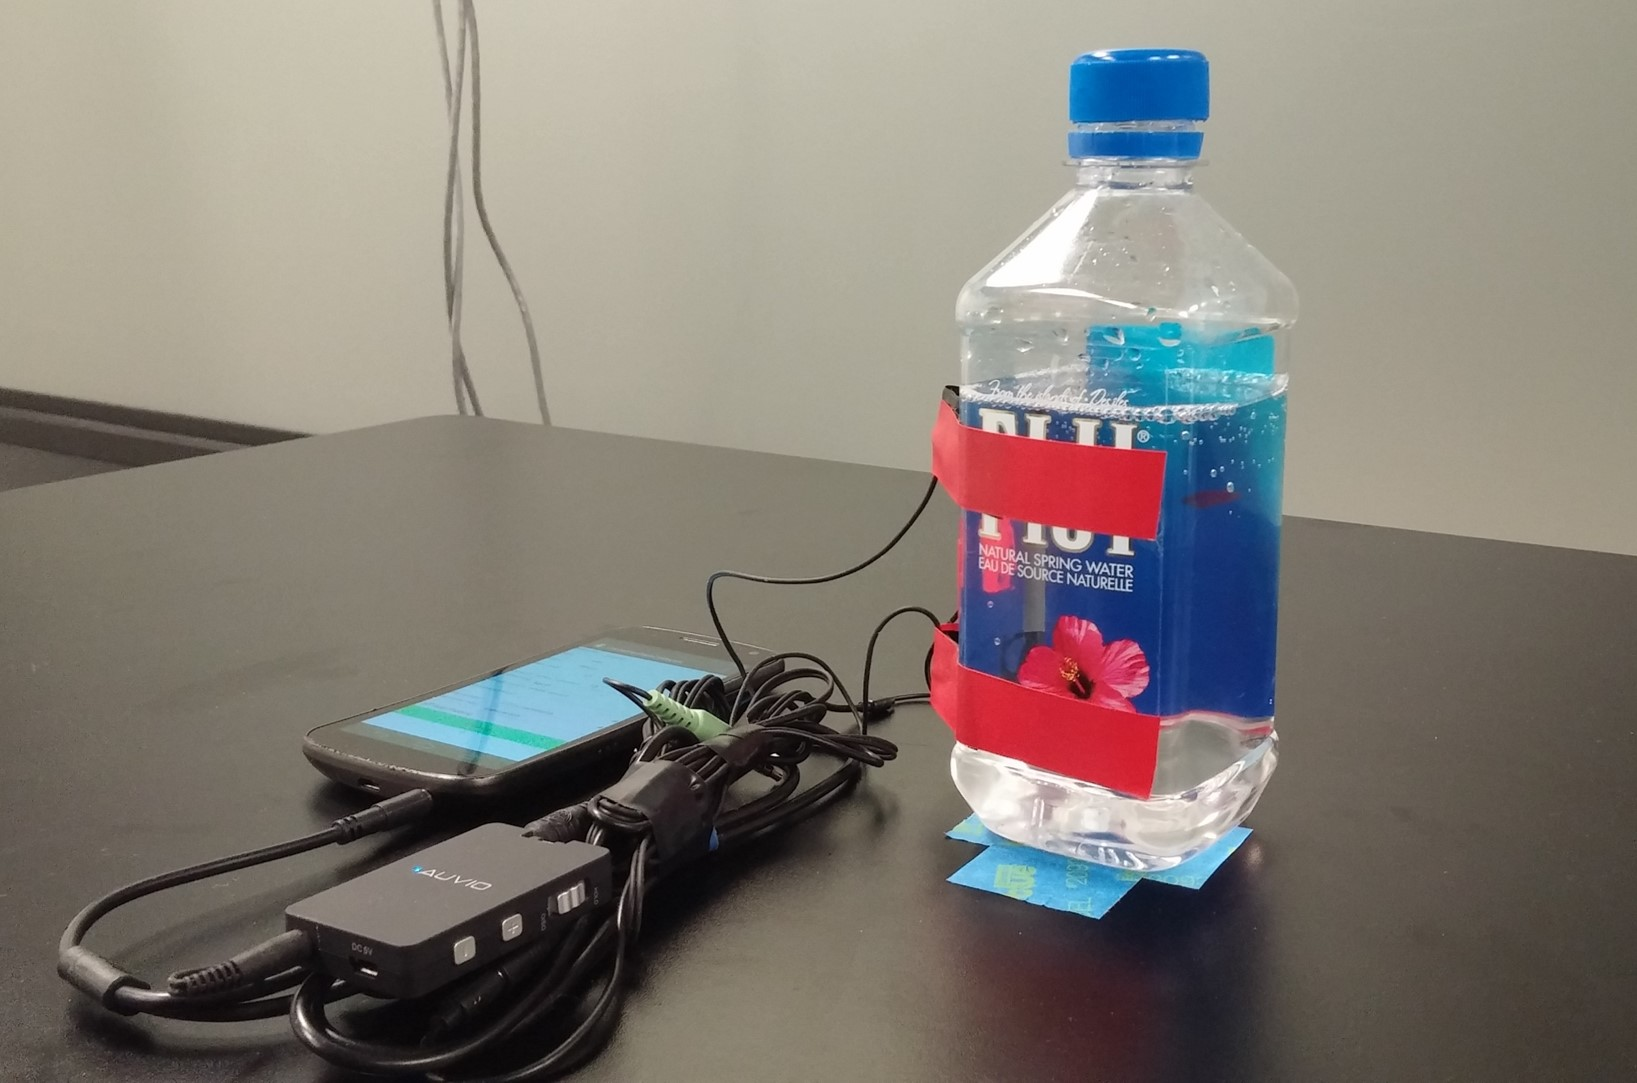
\includegraphics[width=0.5\linewidth]{setup1.jpg}
  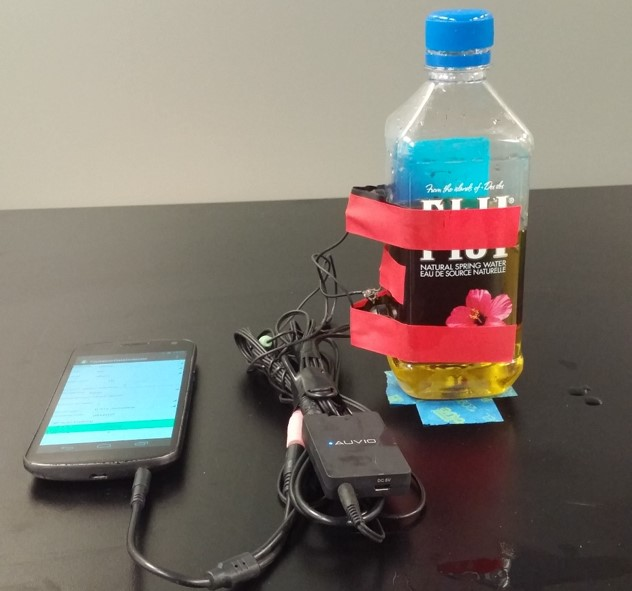
\includegraphics[width=0.242\linewidth]{setup2.jpg}
  \caption{Setup for data collection: the sensor unit is attached to a side surface of a bottle. The unit is connected to an android phone, where a data collection application runs.}
  \label{fig:set-up}
\end{figure}
\begin{figure}[htb]
\centering
\begin{subfigure}{0.32\linewidth}
  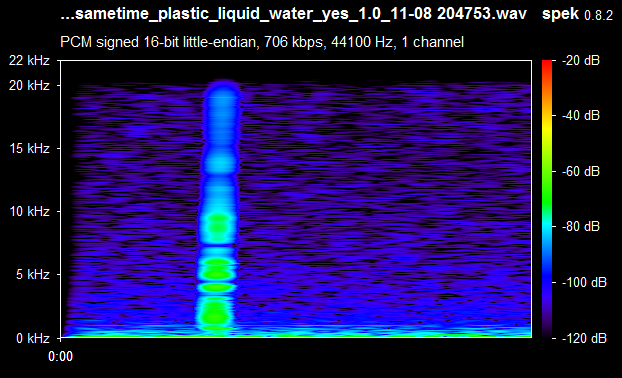
\includegraphics[width=\linewidth]{water_empty.png}
  \caption*{Empty}
\end{subfigure}
\begin{subfigure}{0.32\linewidth}
  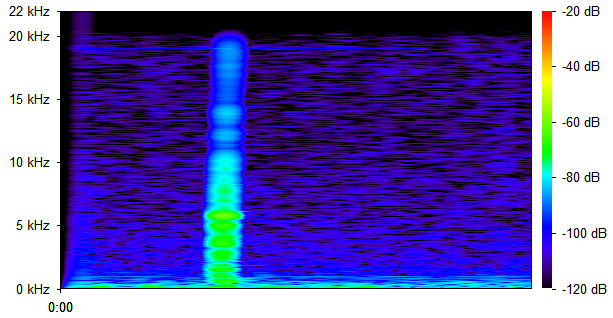
\includegraphics[width=\linewidth]{water_half.png}
  \caption*{Half-filled}
\end{subfigure}
\begin{subfigure}{0.32\linewidth}
  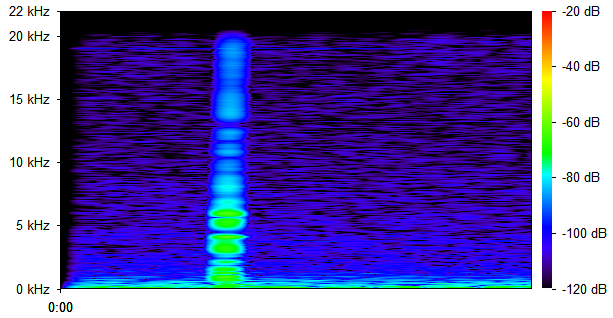
\includegraphics[width=\linewidth]{water_full.png}
  \caption*{Fully filled}
\end{subfigure}
%  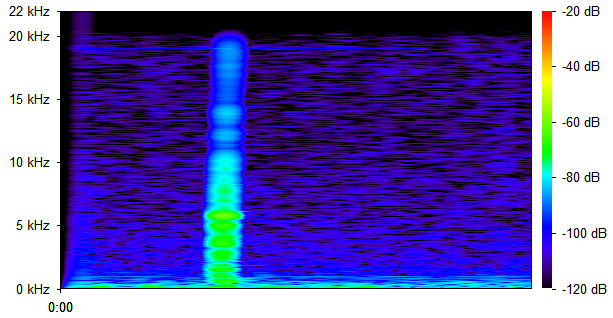
\includegraphics[width=0.3\linewidth]{water_half.png}
%  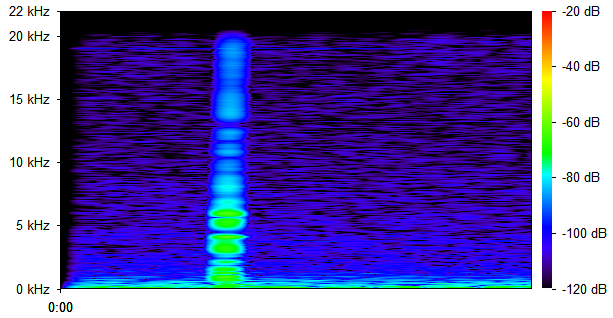
\includegraphics[width=0.3\linewidth]{water_full.png}
  \caption{Spectrograms of impulse response recordings when the bottle contains water.}
  \label{fig:spectrograms}
\end{figure}

We follow the same data collection protocol as we have used in our previous paper~\cite{fan2015soqr}. A brief summary of the data collection steps is presented below.
\begin{enumerate}
\item Choose a liquid for which data has not been collected yet.

\item Start from the empty level. Start the mobile data collection application. The application probes the container and records the impulse response. This is repeated 100 times to suppress the influence of noise.

\item After it finishes data collection for the current level, we measure an amount of the liquid equivalent to 10 percent of the volume of the container and pour this liquid into the container. We wait until the liquid settles and then re-start the mobile application for data collection.

\item We repeat step 3 until the container is fully filled.

\item We clean the container and perform the above 4 steps repeatedly until we finish collecting data samples for all the 9 liquids.

\end{enumerate}

For the data set of each liquid, there are 11 content levels in total and 100 sample audio recordings per content level. Thus, there are 1100 sample recordings per liquid, and a total of 9900 samples for all liquids.

\section{Feature Extraction}
To make use of these raw audio samples, we extract and use the following two types of acoustic features: Mel-frequency cepstral coefficients (MFCCs) and linear predictive coefficients (LPC). MFCCs capture properties of the real cepstral of a short-time signal derived from the fast Fourier transform of an acoustic signal. It has been used for speech recognition and scene understanding~\cite{kunze2007symbolic}~\cite{fan2014public}, etc. LPC calculates the power spectrum of a signal and has been demonstrated efficient for formant analysis and speech analysis. 

To extract these two features, an audio recording is divided into short-time frames using a sliding window of size $W = 512$ samples and 50 percent overlap between two adjacent windows. The output frames are smoothed with a Hamming window function applied and then are converted to frequency domain via fast Fourier transformation. The magnitudes of each frequency bin $k\ (k=1\dots W)$ of a frame $j$ are represented as $\mathtt{FFT}_{j,k}$. We then identify the portion of the recording where the impulse response impacts the most by using the following equation.
\[\argmax_{i\in\{1\dots N\}}\left(\sum_{j=i}^{\min \{i+S, N\}}\sum_{K=0}^{W-1}\mathtt{FFT}_{j,k}\right)\]
where, $S$ is the number of frames during a sweep. That is, $S=(44100*0.01)/(W*50\%)$.

Finally, for the identified portion, we extract 13 MFCCs and 10 LPC for each frame, and them compute the average value of each feature. We remove the first MFCC feature because the distribution of this feature over all levels of any type of liquid are random and. We also remove the last LPC feature because it is always the same for all levels of all liquid types. Therefore, we have 21 features for learning our prediction models.

The range of raw features varies differently for different MFCCs and LPC. This might affect the optimization of our objective functions while training our prediction models. Therefore, we normalize each one of the 21 features using the following standardization equation.
\[\mathbf{x'} = \frac{\mathbf{x}-\overline{\mathbf{x}}}{\sigma(\mathbf{x})}\]
where $\overline{\mathbf{x}}$ represents the mean of a distribution of feature vector $\mathbf{x}$, and $\sigma(\mathbf{x})$ its standard deviation.

\section{Feature Exploration}
In order to explore the viability of a transfer learning approach for adapting or generalizing our models across various liquids, we first ascertained that the various liquid feature {\em domains} showed similar patterns across the quantity levels of the liquid in the container. Figure~\ref{fig:features} visualizes the LPC features for two liquids from the dataset. While we can observe many differences between the features for the two liquids, it is clear that the features follow many similar patterns when observed from the empty level to the full one. Correspondingly, we visualize the distance between the features by scaling them to 2-dimensions using multi-dimensional scaling. The visualization for the same pair of liquids is shown in Figure~\ref{fig:mds}. It can be clearly seen that the features for similar levels occupy similar regions of the MDS manifold surface, irregardless of the liquid.

\begin{figure}[tbh]
\centering
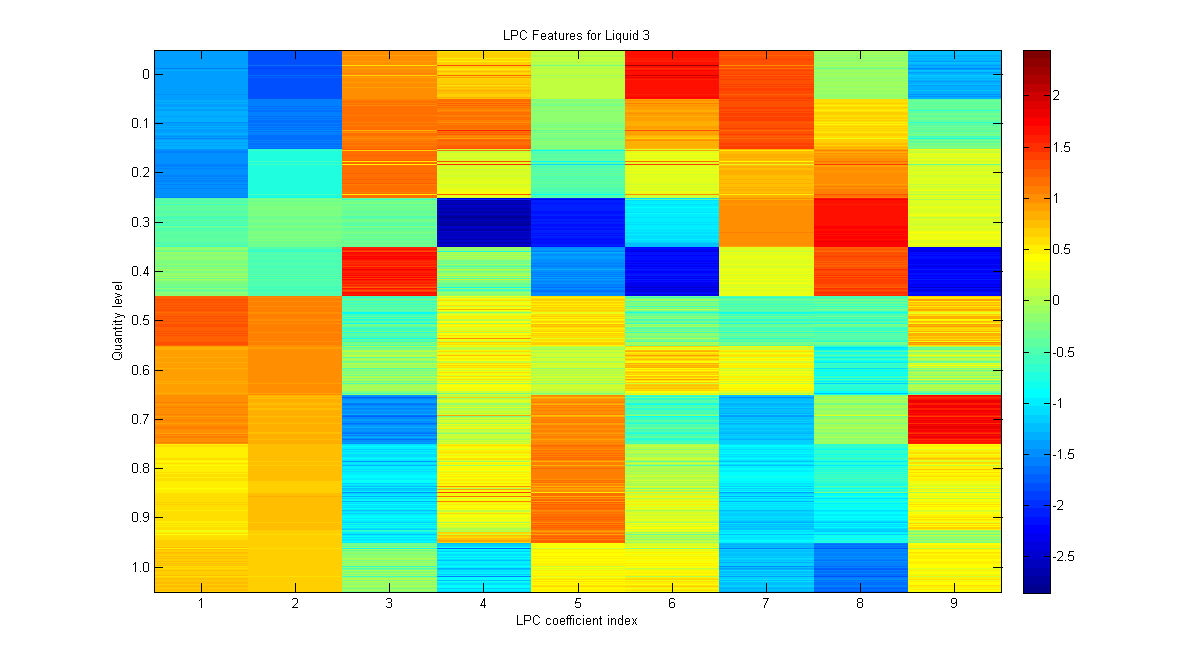
\includegraphics[width=0.49\linewidth]{lpc_3.png}
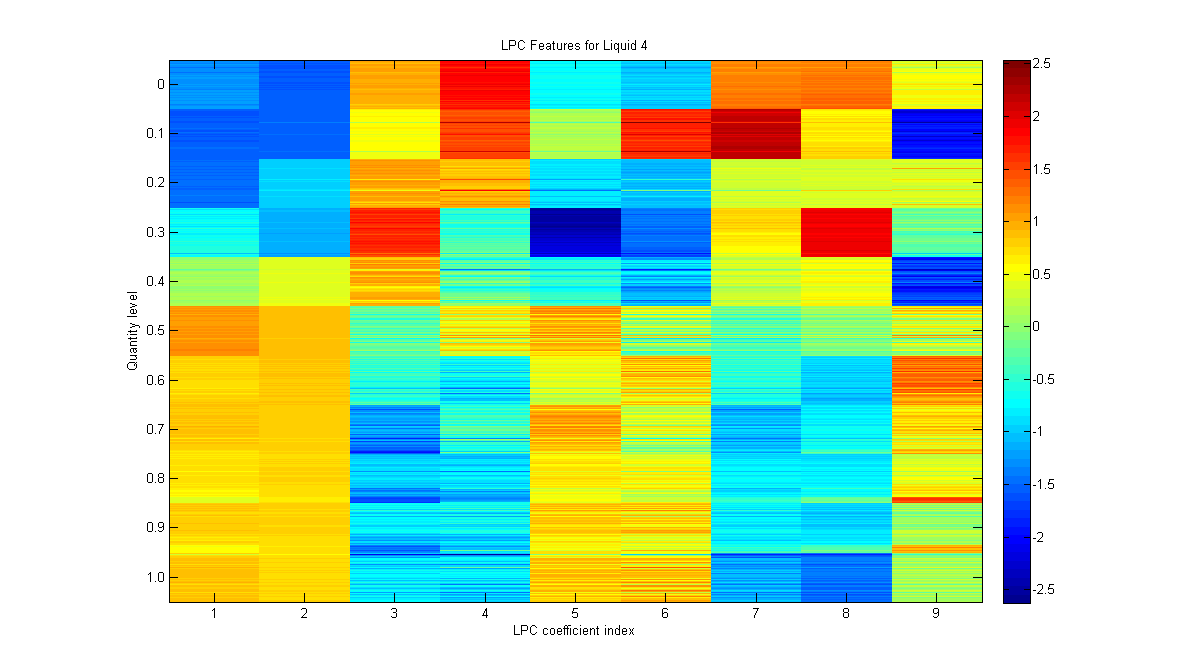
\includegraphics[width=0.49\linewidth]{lpc_4.png}
\caption{Visualizing LPC features for two liquids from the dataset: milk and olive oil.}
\label{fig:features}
\end{figure}

\begin{figure}[htb]
\centering
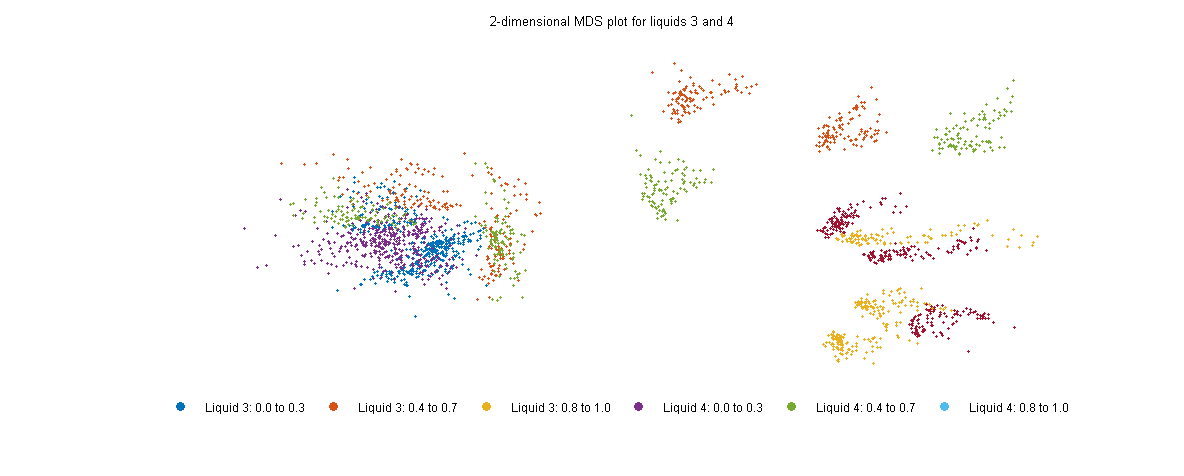
\includegraphics[width=0.8\linewidth]{mds_3_4.png}
\caption{Projecting the features for liquids 3 and 4 of the dataset (milk and olive oil) to a two-dimensional plane using MDS. Note that features representing similar levels are close together in the plane.}
\label{fig:mds}
\end{figure}

\section{Evaluation}
In this section, we report our exploration on the proposed research questions.

\subsection{Research Questions}
We examine the following research questions.

\paragraph{R1} For a given liquid, can we build a classifier that can tell its content level? This question is meant to validate the results that our previous paper has discovered using the new data set we have collected.

\paragraph{R2} Given N (N = 1,...,number of liquid - 1) types of known liquid data and 2 levels (the empty and full levels) of an unknown liquid data, could a prediction model be learned to predict the unknown liquid's content level? If we can build a model, how many types of known liquid we need in order to achieve a decent performance? Put it differently, we want to explore how the prediction model's performance changes as the number of known liquid ($N$) used for training is varied. Do the two levels of the unknown liquid data help improve the prediction model? 


\subsection{Exploration on R1}
The classification problem here is to predict the content level from 11 possible levels (0 to 1 with 10 percent as the interval) given the extracted 21 standardized MFCC and LPC features computed from an impulse response sound clip recorded using our sensor. We train a support vector machine classifier using libSVM~\cite{chang2011libsvm}. For evaluation, we did 10-fold cross validation. The evaluation result is shown in Table~\ref{table:svmEval}. With the data set we collected, we were able to achieve similar performance as~\cite{fan2015soqr}.

\begin{table}[t]
\caption{Evaluation of classification performance of an SVM classifier utilizing RBF kernel.}
\label{table:svmEval}
\begin{center}
\begin{tabular}{ l | c | c | c }
\textbf{LIQUID TYPE} & \textbf{OVERALL PRECISION} & \textbf{OVERALL RECALL} & \textbf{F-MEASURE} \\ \hline
~ & ~ & ~ & ~\\
Apple juice & 0.992 & 0.992 & 0.992 \\
Canola oil & 0.996 & 0.996 & 0.996 \\
Milk & 1.000 & 1.000 & 1.000 \\
Olive oil & 0.998 & 0.998 & 0.998 \\
Orange juice & 0.997 & 0.997 & 0.997 \\
Soy sauce & 0.999 & 0.999 & 0.999 \\
Syrup & 1.000 & 1.000 & 1.000 \\
Tonic water & 0.996 & 0.996 & 0.996 \\
Water & 0.999 & 0.999 & 0.999 \\
\end{tabular}
\end{center}
\end{table}
\subsection{Exploration on R2}
As the prediction class (content level) is a continuous value between 0 and 1, we can treat the prediction as regression.
  
\subsubsection{Ridge Regression}
We use linear regression with Tikhonov regularization, also known as ridge regression to perform
the quantity prediction. Ridge regression regularizes on the 2-norm of the regression parameters,
and has the following least-squares optimization functional.
\[\min_\W\left(\lVert\W\x^T - \mathbf{y}\rVert^2 + \lambda\lVert\W\rVert^2\right)\]
where $\lambda$ is the regularization hyperparameter. Since, this is a convex problem, it can be solved in
the closed form. We use the implementation provided by Yan et al~\cite{yan2015improving} for solving the optimization problem using the normal equation. After empirical analysis, we found that the value of 0.01 for the hyperparameter $\lambda$ gives the best results, and all our results reported in this paper use the same value.

\subsubsection{Artificial Neural Network}
Ridge Regression cannot handle the potential non-linear relation between the features and the target value. To cope with this problem, we further explored a non-linear regression model: artificial neural network. Specifically, we adopted a Multi-Layer Perceptron (MLP), which is a feed-forward artificial neural network model. By having nonlinear activation functions, MLP can distinguish the data that is not linearly separable. 

We designed an MLP with one input layer of 21 nodes, one output layer with 1 node to output the prediction result, and 2 hidden layers in between. We chose 2 hidden layers for the following reasons. We expected the nodes in the first hidden layer to learn more complex and informative features based on the input features. We expected the second hidden layers to learn the latent variables that determine the content level. In our case, the hidden variables are physical properties that could affect the sound absorption and reflection while traveling through the liquid. For the number of nodes in the first hidden layer, we chose (21 + 11)/2 for the first hidden layer (21 is the dimension of the input feature vector and 11 is the number of target values) by following the guidance of MLP design in a machine learning and data mining toolkit WEKA~\cite{hall2009weka}. It proposes the number of nodes for the hidden layer can be chosen as $(\#attributes + \#classes) / 2$. For the number of nodes in the second hidden layer, we chose the value as 4 in the hope of simulating the 4 major physical properties introduced earlier, namely viscosity, specific heat, density, and temperature, which affect sound absorption and refection in liquids. To handle the non-linearity, we used a sigmoid function as the activation function. The MLP is visualized in Figure~\ref{fig:network}. All the nodes in one layer are fully connected to the nodes in the next layer. The output of the final layer is the linear combination of its inputs multiplied by their weights.

\begin{figure}[tbh]
\centering
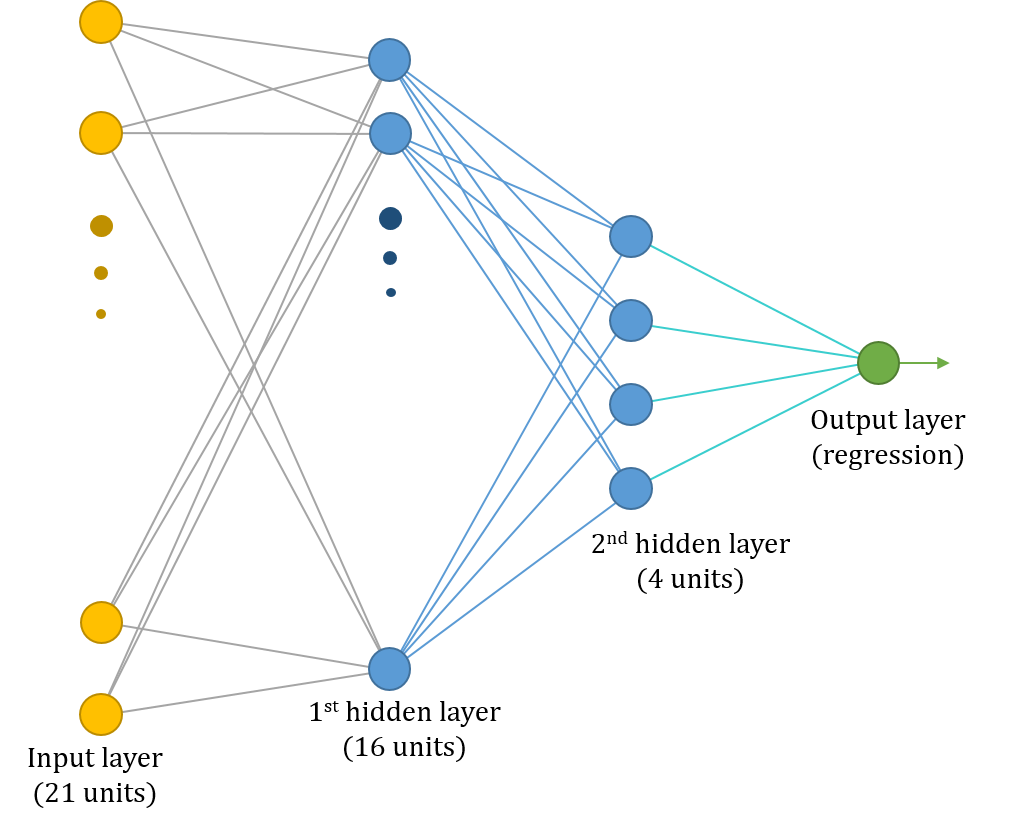
\includegraphics[width=0.75\linewidth]{network.png}
\caption{Multi-layer perceptron used for the experiments. Note that all the layers are fully connected.}
\label{fig:network}
\end{figure}
We used squared-error loss function.\begin{equation} E=(f(x)-y)^2/2\end{equation} We used back-propagation algorithm, which is a fast way of computing gradients, to learn all the weights in the MLP. We used a mini-batch size of 100 while learning the weights. We also tuned the following parameters: learning rate, momentum, the number of epochs trained. Based on the empirical results, we finally set these parameters to be 0.3,0.2 and 2000.


\subsubsection{Evaluation Strategy}
We used the mean absolute error (MAE) to evaluate the performance of two prediction models: Ridge Regression and MLP. We train each regression model using the combined data set of $N$ ($N = 1\dots \#liquids - 1)$ known liquid and 2 levels (full and empty levels) of unknown liquid data. To examine how a regression model's performance change when the number of known liquid used for training increases, we gradually increase the number of liquid used from 1 to 8 (9 is the total number of liquid we have). If we use $N$ liquids for training, then we will test the model on each of the remaining $9-N$ liquids. Therefore, the number of rounds of evaluations for for models trained with $N$ liquids' data can be expressed as $C_N^9 * (9-N), N = 1\dots 8$. For example, the number of rounds of evaluations for the models trained with 5 liquids' data is $C^9_5 * (9-5) = 630$.

For a regression model and the number of liquids used for training, $N$, we compute the MAE for each round of evaluation $e_i$, where $i= 1\dots C_N^9 * (9-N)$ and compute the mean and the standard deviation of $e_i$.

\subsubsection{Reweight Samples}
While training a regression model, we use data from $N$ liquids and also data from 2 levels (empty and full) of the unknown liquid that our model is going to predict content level on. One strategy is simply combining them together and train the model, which is named $\mathtt{Strategy}^1$. 

One potential problem with this strategy is that the number of samples from $N$ types of liquid $(N * 1100)$ is normally much higher than the number of samples from the 2 levels of the unknown liquid (200). For example, if we train the regression model with $N = 8$ liquids, we have 8800 samples from the known liquid but only 200 samples from the unknown liquid. The effect of these 200 samples might be "washed" out by those 8800 samples. To tackle this problem, we proposed a reweight method: if $N$ liquids are used for training, then we will duplicate the 200 samples from the unknown liquid by $N$ times. Thus, there will be $N * 1100 + N * 200$ samples for training. We name this strategy as $\mathtt{Strategy}^2$.

\begin{table}[t]
\caption{Overall regression performance: mean absolute error in quantity level prediction for various source set sizes.}
\label{table:result}
\begin{center}
\begin{tabular}{ l | c | c | c | c}
\textbf{\# SRC LIQUIDS} & \multicolumn{2}{c|}{$\mathtt{Strategy}^1$} & \multicolumn{2}{c}{$\mathtt{Strategy}^2$} \\ \hline
~ & ~ & ~ & ~ & ~\\
~ & \textbf{Ridge} & \textbf{MLP} & \textbf{Ridge} & \textbf{MLP}\\ \hline
~ & ~ & ~ & ~ & ~\\
1 & 0.141 & \textbf{0.097} & 0.141 & \textbf{0.097}\\
2 & 0.120 & \textbf{0.078} & 0.117 & 0.081\\
3 & 0.110 & \textbf{0.074} & 0.107 & \textbf{0.074}\\
4 & 0.107 & \textbf{0.069} & 0.102 & 0.076\\
5 & 0.105 & 0.073 & 0.100 & \textbf{0.069}\\
6 & 0.104 & \textbf{0.066} & 0.098 & 0.067\\
7 & 0.103 & \textbf{0.066} & 0.097 & 0.073\\
8 & 0.102 & 0.063 & 0.096 & \textbf{0.062}\\
\end{tabular}
\end{center}
\end{table}

\subsubsection{Results}
In this section, we show the results of the two regression models (Ridge regression and MLP) using two Reweight samples strategies ($\mathtt{Strategy}^1$,$\mathtt{Strategy}^2$). The overall results are described in Table~\ref{table:result}. Note that all training processes include the 2 level data (empty and full levels) from the testing liquid.

\begin{itemize}
\item Figure~\ref{fig:ridge} shows the performance of the two re-weighting strategies using ridge regression model. The X-axis is the number of liquids used for training.

\item Figure~\ref{fig:nn} shows the performance of the two re-weighting strategies using a multi-layer perceptron. The X-axis is the number of liquid used for training.

\item Figure~\ref{fig:water} shows the predictions made by the two models when tested on water, and trained using all the other liquids using the $\mathtt{Strategy}^2$ strategy. This particular testcase presented the best results in our dataset for both the models.
\end{itemize}


\begin{figure}[htb]
\centering
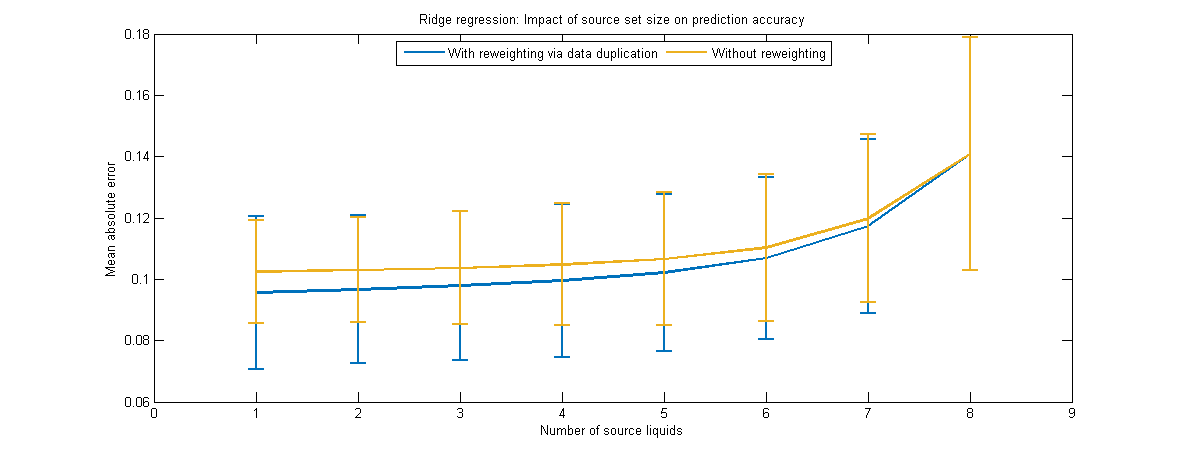
\includegraphics[width=\linewidth]{source_set_size_ridge.png}
\caption{Ridge regression prediction results.}
\label{fig:ridge}
\end{figure}

\begin{figure}[htb]
\centering
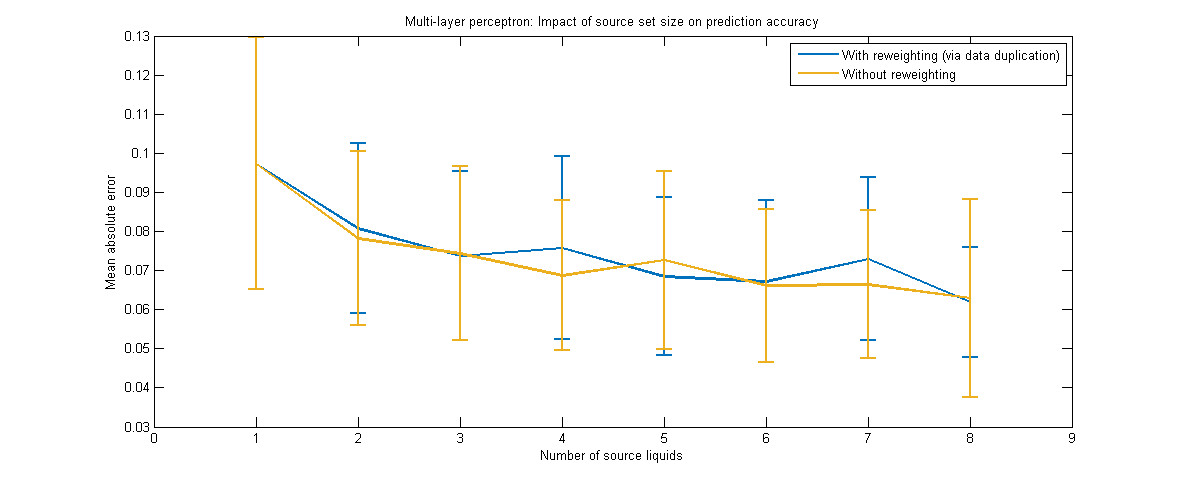
\includegraphics[width=\linewidth]{source_set_size_nn.png}
\caption{Multi-layer perceptron prediction results.}
\label{fig:nn}
\end{figure}

\begin{figure}[htb]
\centering
\begin{subfigure}{\linewidth}
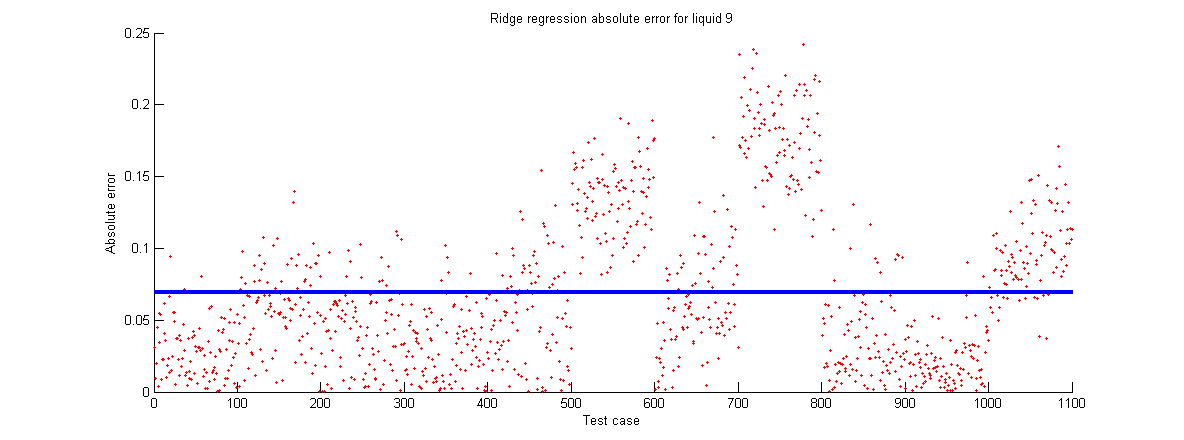
\includegraphics[width=0.49\linewidth]{train1-8_test9_regress.png}
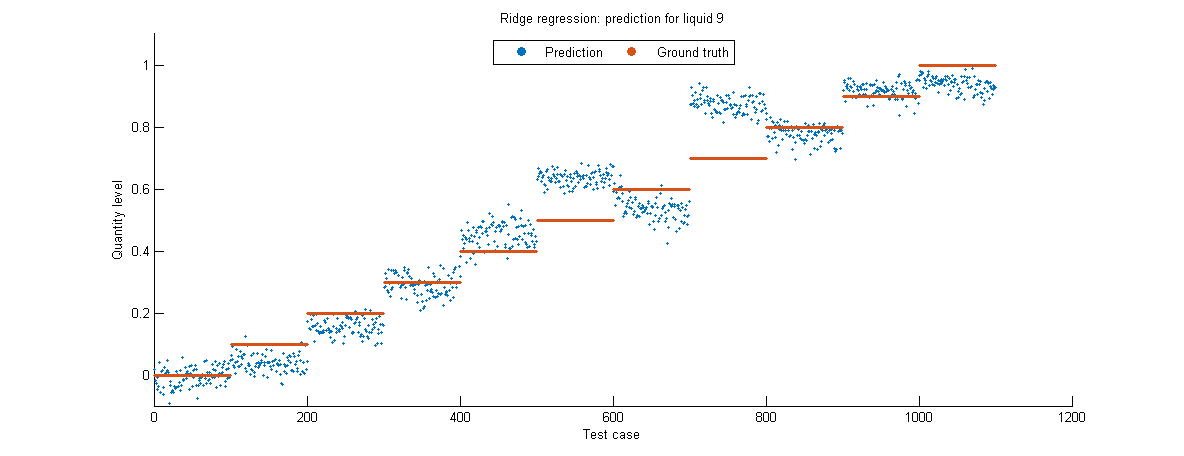
\includegraphics[width=0.49\linewidth]{train1-8_test9_regress_prediction.png}
\caption*{Ridge regression}
\end{subfigure}
\begin{subfigure}{\linewidth}
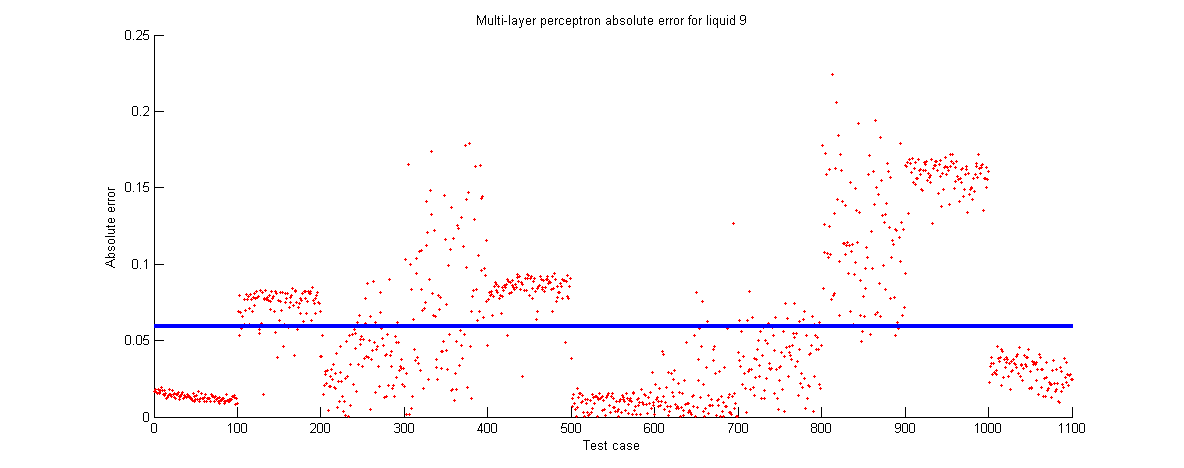
\includegraphics[width=0.49\linewidth]{train1-8_test9_nn.png}
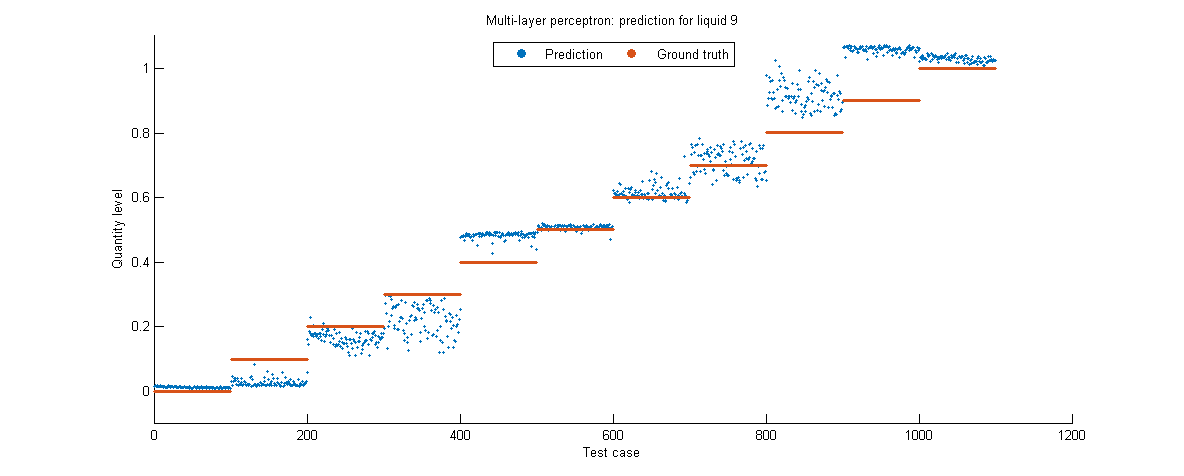
\includegraphics[width=0.49\linewidth]{train1-8_test9_nn_prediction.png}
\caption*{Multi-layer perceptron}
\end{subfigure}
\caption{Prediction results targeting the liquid {\em water}, while using all other liquids used as sources for domain adaptation. Both the models use $\mathtt{Strategy}^2$. The blue line in the left column represents the mean absolute error.}
\label{fig:water}
\end{figure}




\section{Conclusion}
In this paper, we tackle a domain adaption problem by learning a regression model to predict the content level of a new type of liquid based on a number of known types of liquid data stored in the same container. Our exploration demonstrate the following three findings: 
\begin{enumerate}
\item It is possible to build a decent regression model to predict the content level of a new type of liquid based only on a number of known types of liquid and 2 levels (empty and full) of the predicting liquid.

\item The MLP model performs better than the ridge regression model if trained on the same data set.

\item Reweighting 2 levels of the predicting liquid data helps improve the model's performance of the ridge regression model. However, it does not seem to help improve the MLP's performance a lot.

\item As the number of liquid used for training increases, both ridge regression and MLP performance improve. For MLP model, when trained on 4 types of liquid, the model's performance become roughly stable (MAE is around 0.07).   
\end{enumerate}

In addition, we evaluated a MLP model trained on 1 type of liquid data and the 2 level data from the testing liquid and compared to another MLP model trained on the same type of liquid data and without the 2 level data from the testing liquid. The MAE for these two cases are: 0.06 and 0.1773. Though not a thoroughly evalution, it shows that the two levels from the testing liquid helps the MLP model trained on existing liquid adapting to the new liquid.  

\subsubsection*{Acknowledgments}
We thank Shikhar Sharma and Prof. Khai Truong for various helpful discussions and ideas.


\bibliography{report}
\bibliographystyle{plain}
\end{document}
